\documentclass[a4paper, 12pt, final, garamond]{book}
\usepackage{cours-preambule}

\makeatletter
\renewcommand{\@chapapp}{Devoir surveill\'e -- num\'ero}
\makeatother

\begin{document}
\setcounter{chapter}{3}

\def\lspace{25}

\chapter{Commentaires sur le DS \oldno4}

\section{Commentaires généraux}
\subsection{Appréciation globale}
\subsection{Sur la forme}
Numérotez les \textbf{copies} et pas les pages, et numérotez les copies en
donnant le nombre de copie maximal~! Copie 1 $\Ra$ et alors~? Copie 1/2 $\Ra$
il existe une autre copie. À savoir et à ne pas manquer.

\subsection{Commentaires principaux et récurrents}

% \begin{figure}[htbp!]
% 	\centering
% 	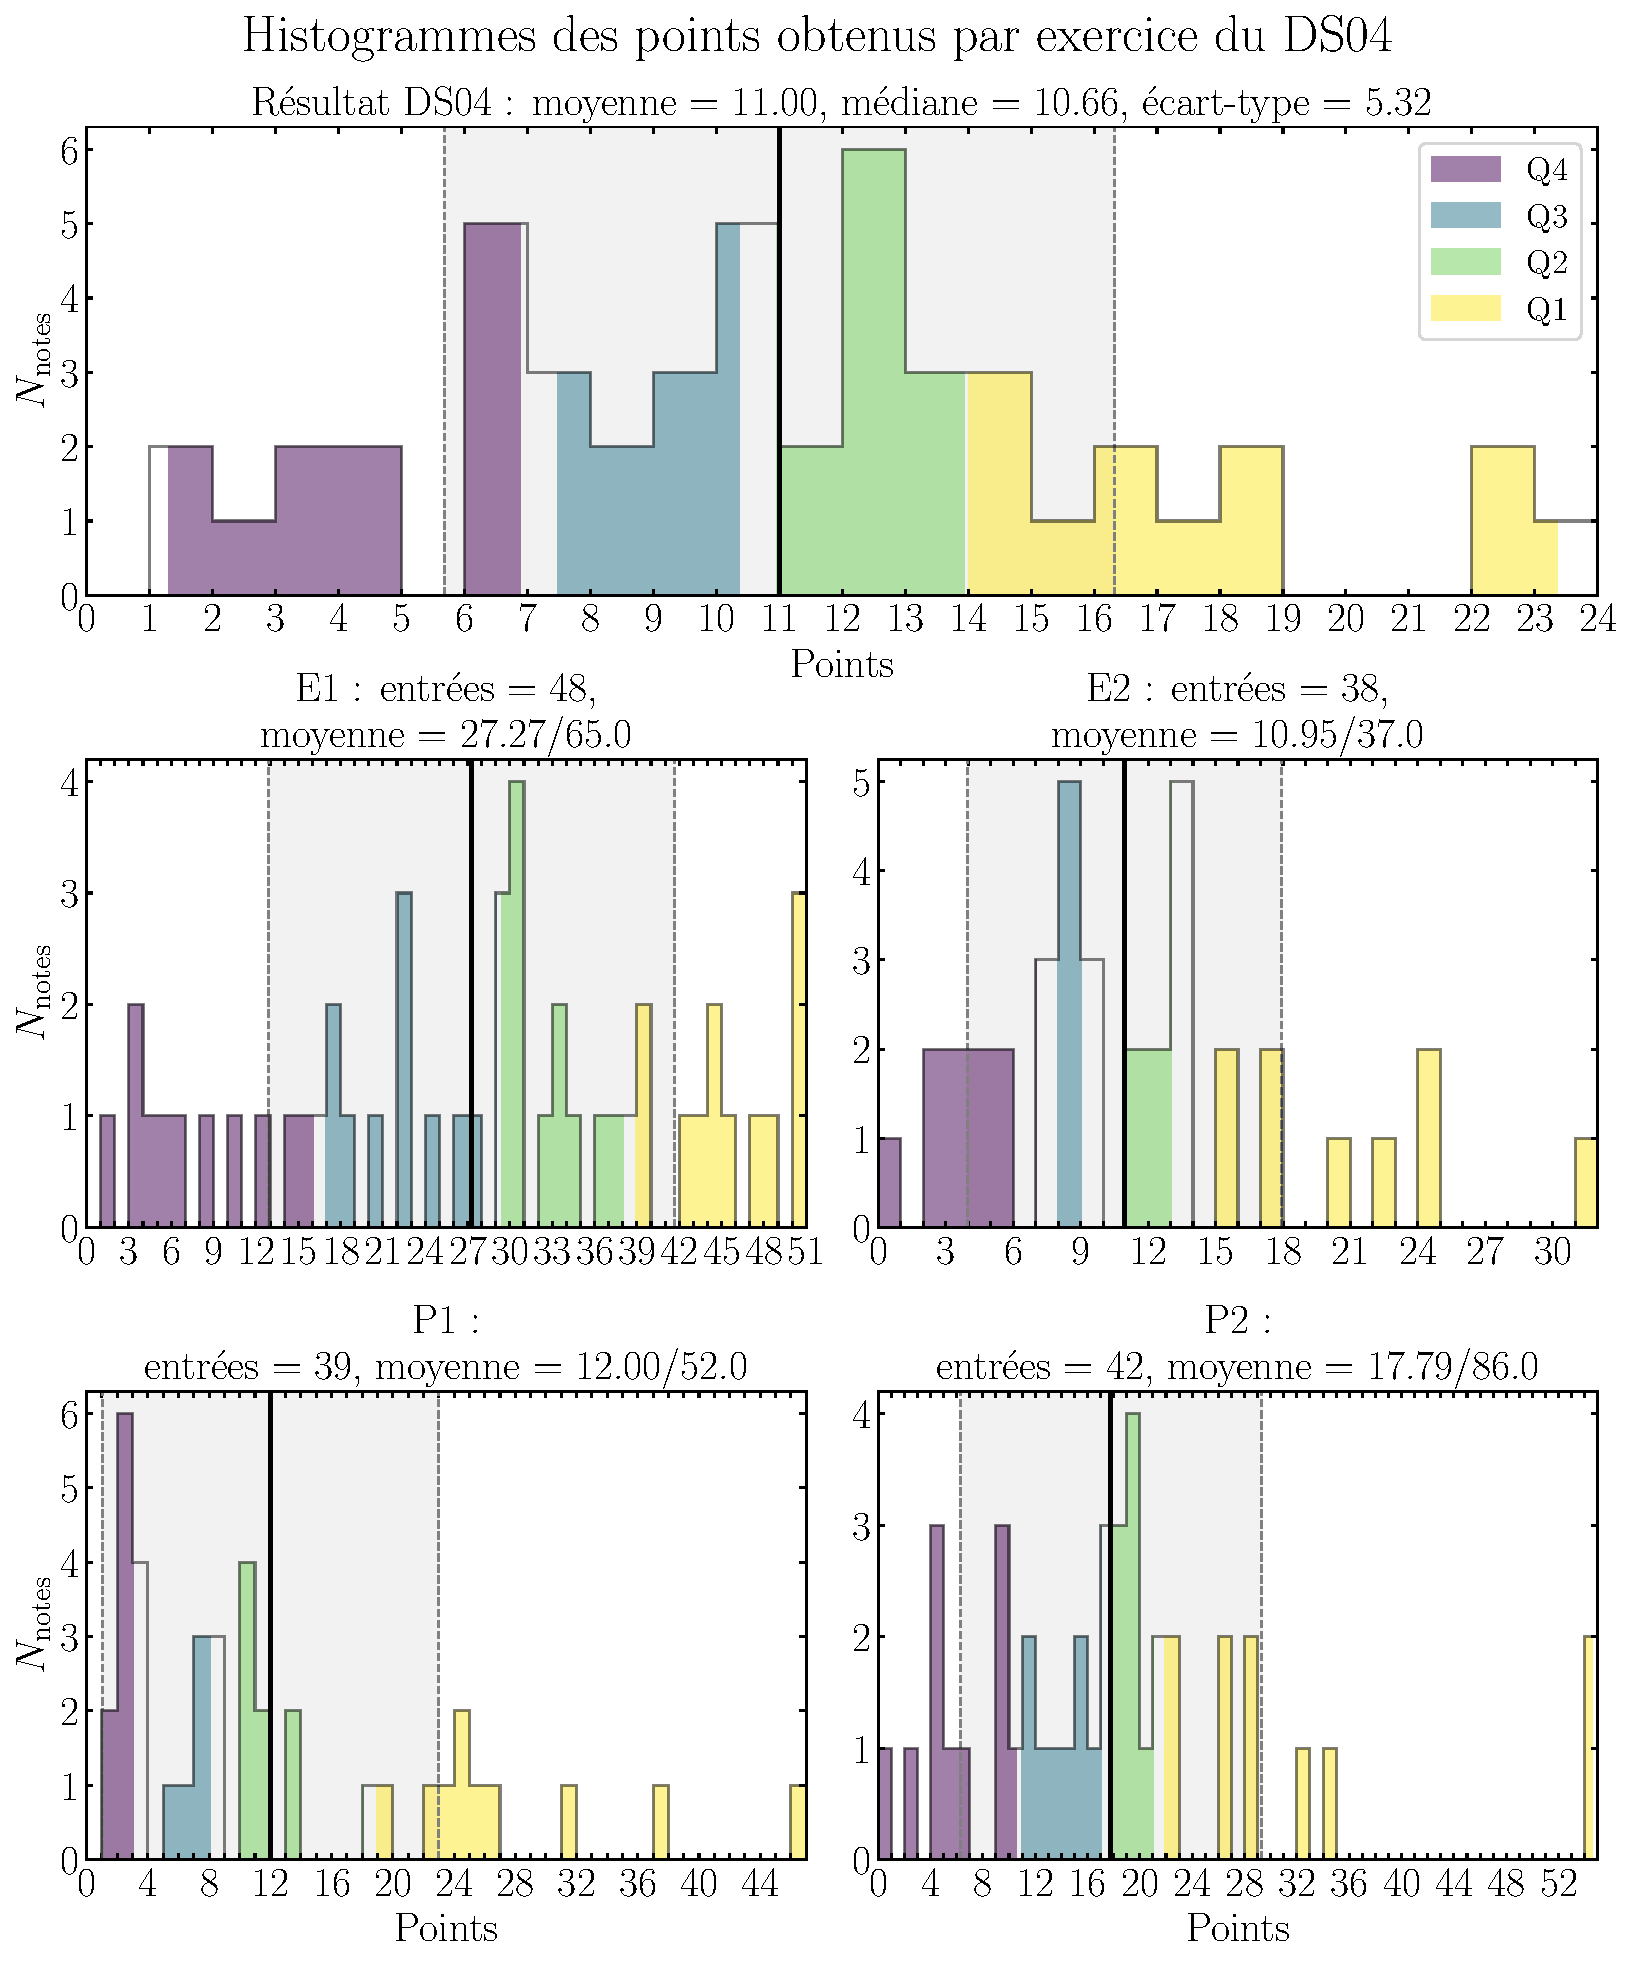
\includegraphics[width=\linewidth]{DS04_hist_all}
% 	\caption{Graphique des résultats}
% \end{figure}

\setcounter{section}{0}
\section[65]"E"{Étude d'un circuit RLC parallèle}
\begin{enumerate}
	\item[n]{3} % Q1
	      Ça ne sert à rien d'ajouter les admittances 2 par 2~! Si vous avez 3
	      impédances en série, vous faites $\Zu = \Zu_1+\Zu_2+\Zu_3$. Pour 3
	      impédances en parallèle, $\Yu = \Yu_1+\Yu_2+\Yu_3$~!
	\item[n]{5} % Q2
	      Répondez à la question~: donnez $\w_0$ et pas $\w_0{}^2$.
	      \textbf{Identifiez}. Gros problèmes d'identification…
	\item[n]{2} % Q3
	      N'oubliez pas la racine carrée~!
	\item[n]{8} % Q4
	      Résonance = amplitude max \textbf{pour $\boxed{\w \neq 0}$}~!
	\item[n]{8} % Q5
	      La bande passante c'est une différence de \textbf{pulsations} (ou
	      fréquences), donc vous ne pouvez pas écrire
	      \[
		      \Delta{\w} = \frac{U\ind{max}}{\sqrt{2}}
		      \quad \red{\circled{$-$H}}
	      \]
	      Il faut mettre les trinômes \textbf{sous forme de trinôme}~!
	      \[
		      \boxed{a x^2 + b x + c = 0}
		      \qMath{et pas}
		      \cancel{ax + \frac{b}{x} + c = 0}
	      \]
	\item[n]{7} % Q6
	      Tracez, bon sang~!
	\item[n]{6} % Q7
	      \leavevmode\vspace*{-15pt}\relax
	      {\Large
		      \[
			      \boxed{\f \neq \phi \neq \Phi \neq \varnothing}
			      \quad \text{!}
		      \]
	      }
	\item[n]{5} % Q8
	\item[n]{4} % Q9
	      Horrible, horrible représentation du courant $\eta$ sur le schéma. Il a
	      échappé à ma vigilance. Je vous présente mes excuses pour vos yeux
	      meurtris.
	\item[n]{5} % Q10
	\item[n]{5} % Q11
	\item[n]{2} % Q12
\end{enumerate}

\section[37]"E"{Monoxyde et dioxyde d'azote}
\begin{enumerate}
	\item[n]{6} % Q1
	      Il y a 4 fois plus de diazote que d'oxygène dans l'air. Cf.\ premier
	      exercice de TDTM2\_app.
	\item[n]{11} % Q2
	      Il faut voir que la réaction était quasi-nulle~!
	\item[n]{7} % Q3
	      Constante de réaction $K^\circ \neq k$ constante de vitesse…
	      Retour sur les confusions entre favorisé et sens de réaction
	\item[n]{4} % Q4
	      Vous êtes tombé-es dans le panneau. On trace $\ln (v)$, ça na \textbf{rien à
		      voir} avec $\ln c(t)$. \textbf{La méthode différentielle} ($\ln (v)$) n'est
	      \textbf{pas la méthode intégrale} (régressions variées).
	\item[n]{4} % Q5
	      Les vitesses $v_1$ et $v_2$ sont différentes~! Ça se voit avec les
	      régressions. Ne partez pas d'une égalité clairement fausse.
	\item[n]{2} % Q6
	      Les proportions stœchiométriques n'ont \textbf{RÀV} avec le fait que les
	      ordres partiels soient ou non égaux aux coefficients stœchiométriques.
	\item[n]{3} % Q7
\end{enumerate}

\setcounter{section}{0}
\section[52]"P"{Suivi cinétique de la formation du dibrome}
\begin{enumerate}
	\item[n]{2} % Q1
	      Bien.
	\item[n]{8} % Q2
	      Faire un schéma pour montrer que chaque concentration est divisée par 2~!
	      Cf.\ TP11… Faites des tableaux d'avancement~!
	\item[n]{6} % Q3
	\item[n]{13} % Q4
	\item[n]{9} % Q5
	\item[n]{2} % Q6
	\item[n]{9} % Q7
	\item[n]{3} % Q8
\end{enumerate}

\section[86]"P"{Résonance d'un verre}
\begin{enumerate}
	\item[n]{5} % Q1
	      Faites un effort sur les chiffres significatifs sur votre lecture…
	\item[n]{10} % Q2
	      Encore une fois, c'est $\ux$ et pas $\vv{x}$~!! Décomposez entièrement
	      les forces sur les vecteurs de base $\ux$ et $\uy$. \textbf{N'inventez
		      pas des conditions initiales} si elles ne sont pas données.
	      \smallbreak
	      Lisez bien l'énoncé~: $\ell_0 = 0$~! Même pas besoin de changement de
	      variable, $x(t)$ c'est déjà $\ell(t)$.
	      \smallbreak
	      Un axe c'est une droite, $Ox$ par exemple, mais $Ox$ a l'unité d'une
	      distance~; un vecteur de base c'est $\ux$, qui est \textbf{u}nitaire,
	      pas d'unité. Donc $\dcancel{\vv{Ox}}$~!
	\item[n]{5} % Q3
	      \leavevmode\vspace*{-15pt}\relax
	      \begin{itemize}
		      \item Écrivez le PFD en version \textbf{vectorielle} avant toute
		            potentielle écriture en colonnes.
		      \item Quand vous \textbf{projetez} sur $\ux$, il ne reste \textbf{que
			            des scalaires}~! Vous ne pouvez pas écrire
		            \begin{gather*}
			            \beforetext{Sur $\ux$}
			            \vv{f} + \vv{F_r} = m \af
		            \end{gather*}
		            La relation vectorielle n'est vrai que pour la somme de tous les
		            vecteurs, vous ne pouvez pas extraire une partie de l'équation.
		            C'est comme si vous écriviez
		            \begin{gather*}
			            a+b = c+d
			            \\\beforetext{donc j'extrait}
			            b = d
		            \end{gather*}
		      \item Identifiez $Q$ et $\w_0$~!
	      \end{itemize}
	\item[n]{3} % Q4
	\item[n]{9} % Q5
	      Frottements faibles $\neq$ frottements nuls~!
	\item[n]{4} % Q6
	\item[n]{4} % Q7
	\item[n]{2} % Q8
	\item[n]{5} % Q9
	\item[n]{4} % Q10
	\item[n]{2} % Q11
	\item[n]{4} % Q12
	\item[n]{3} % Q13
	\item[n]{10} % Q14
	\item[n]{2} % Q15
	\item[n]{2} % Q16
	\item[n]{7} % Q17
	\item[n]{5} % Q18
\end{enumerate}

\end{document}
